% ju 11-Jun-22
\documentclass[a4paper,12pt,fleqn,parskip=half]{scrartcl}
\usepackage[ngerman]{babel}
\usepackage[utf8]{inputenc}
\usepackage[T1]{fontenc}

% Schrift
%\usepackage{lmodern}
\usepackage[osf,sc]{mathpazo} 
\usepackage[scale=.9,semibold]{sourcecodepro}   
\usepackage[osf]{sourcesanspro}  

\usepackage[headsepline]{scrlayer-scrpage}
\pagestyle{scrheadings}
\clearpairofpagestyles

\usepackage[table,dvipsnames,usenames]{xcolor}
\usepackage{textcase}
\usepackage{nameref}
\usepackage{hyperref}
\usepackage{tabularx}
\usepackage{multirow}
\usepackage{multicol}
\usepackage{caption, booktabs}
\usepackage{graphicx} 
\usepackage{scrhack}    
\usepackage{url}%% Links
\usepackage[inline]{enumitem}
\usepackage{pifont}
\usepackage{eurosym}% \euro 20,-
\usepackage{amsmath}
\usepackage{amsfonts}
\usepackage{amssymb}
\usepackage{array}            % Extending the array and tabular environments
\usepackage{chngcntr}         % Change the resetting of counters
\usepackage[version=4]{mhchem}
\usepackage{stmaryrd}
\usepackage{siunitx}
\usepackage{float}
\usepackage{csquotes}
\usepackage{subcaption}
\usepackage{mathtools}
\usepackage{icomma}%Dezimaltrennzeichen
\usepackage{multimedia}%Video: \movie[externalviewer]{(video.mov)}{video.mov}
\usepackage{epstopdf}
\usepackage{footnote}
\usepackage{qrcode}% Anwendung: \qrcode[hyperlink,level=Q,version=2,height=1cm]{\website}
\usepackage{underscore}% Unterstrich ____

% PDF Dokumente einbinden
\usepackage{pdfpages}% \includepdf[pages=-]{Tabellen/Excel.pdf}
\RequirePackage{lastpage}  % Pagecounter

\addto\captionsngerman{%
\renewcommand{\figurename}{Abb.}
\renewcommand{\tablename}{Tab.}
}

% listings
\usepackage{listings}
\lstset{basicstyle=\linespread{1}\ttfamily\small,floatplacement=!htb,captionpos=t,abovecaptionskip=.5\baselineskip,belowcaptionskip=.5\baselineskip,upquote=true,showstringspaces=false,inputencoding=utf8,tabsize=4,
    	keywordstyle=\bfseries ,
	commentstyle=\color{rot5},
	stringstyle=\color{orange},
	breaklines=true,
  	postbreak=\mbox{\textcolor{black}{$\hookrightarrow$}\space},
	breakatwhitespace=false
}
\lstset{literate={á}{{\'a}}1 {é}{{\'e}}1 {í}{{\'i}}1 {ó}{{\'o}}1 {ú}{{\'u}}1 {Á}{{\'A}}1 {É}{{\'E}}1 {Í}{{\'I}}1 {Ó}{{\'O}}1 {Ú}{{\'U}}1 {à}{{\`a}}1 {è}{{\`e}}1 {ì}{{\`i}}1 {ò}{{\`o}}1 {ù}{{\`u}}1 {À}{{\`A}}1 {È}{{\'E}}1 {Ì}{{\`I}}1 {Ò}{{\`O}}1 {Ù}{{\`U}}1 {ä}{{\"a}}1 {ë}{{\"e}}1 {ï}{{\"i}}1 {ö}{{\"o}}1 {ü}{{\"u}}1 {Ä}{{\"A}}1 {Ë}{{\"E}}1 {Ï}{{\"I}}1 {Ö}{{\"O}}1 {Ü}{{\"U}}1 {â}{{\^a}}1 {ê}{{\^e}}1 {î}{{\^i}}1 {ô}{{\^o}}1 {û}{{\^u}}1 {Â}{{\^A}}1 {Ê}{{\^E}}1 {Î}{{\^I}}1 {Ô}{{\^O}}1 {Û}{{\^U}}1 {œ}{{\oe}}1 {Œ}{{\OE}}1 {æ}{{\ae}}1 {Æ}{{\AE}}1 {ß}{{\ss}}1 {ű}{{\H{u}}}1 {Ű}{{\H{U}}}1 {ő}{{\H{o}}}1 {Ő}{{\H{O}}}1 {ç}{{\c c}}1 {Ç}{{\c C}}1 {ø}{{\o}}1 {å}{{\r a}}1 {Å}{{\r A}}1 {€}{{\EUR}}1 {£}{{\pounds}}1 {~}{{\textasciitilde}}1 {-}{{-}}1 }

% bibliography
\usepackage[
    bibencoding=utf8,
    backend=biber,% bibtex, biber
    backref=false,backrefstyle=three+,url=true,urldate=comp,abbreviate=false,maxnames=20
]{biblatex} %Paket laden
\DeclareBibliographyCategory{cited}
\let\defaultcite\cite\renewcommand*\cite[2][]{\addtocategory{cited}{#2}\defaultcite[#1]{#2}}
\let\defaulttextcite\textcite\renewcommand*\textcite[2][]{\addtocategory{cited}{#2}\defaulttextcite[#1]{#2}}
\setcounter{biburllcpenalty}{7000}
\setcounter{biburlucpenalty}{8000}
\AfterPackage{biblatex}{
	\PreventPackageFromLoading[\errmessage{Sie haben versucht, das Cite-Paket zu laden, das nicht mit biblatex kompatibel ist.}]{cite}
}

\hypersetup{%
	%pdftitle={\titel},
	%pdfsubject={Latex},
	%pdfauthor={\autor},
	%pdfcreator={\autor}, 
	bookmarksnumbered=true,
	breaklinks=true,
	%colorlinks=true,	   
	linkcolor=rot5,		
	filecolor=blau5,		
	urlcolor=blau5,			
	citecolor=ForestGreen
}

\linespread{1.1}
\setlist{itemsep=0pt}
\widowpenalty10000
\clubpenalty10000
\tolerance1000   

\usepackage[left=2cm,right=2cm,top=1cm,bottom=1cm,includeheadfoot]{geometry}
%\usepackage[left=4cm,right=2cm,top=1cm, bottom=1cm,includeheadfoot]{geometry}
%\usepackage[left=6cm,right=1cm,top=1cm, bottom=1cm,includeheadfoot]{geometry}
%\usepackage[landscape=true,left=2cm,right=2cm,top=1cm,bottom=1cm,includeheadfoot]{geometry}%quer

% eigene Farbe definieren
% Adobe Prozessfarben: CMYK: 100,50,0,35 -> 1,0.5,0,0.35
\definecolor{orange}{cmyk}{0,0.55,0.61,0}   % 0,55,61,0
\definecolor{blau5}{cmyk}{1,0.77,0.1,0.01}  % 100,77,10,
\definecolor{rot5}{cmyk}{0.22,1,1,0.19}     % 22,100,100,19
\definecolor{grau2}{cmyk}{0,0,0,0.1}        % 0,0,0,40
\definecolor{blau}{cmyk}{0.93,0.66,0,0.21}% 

% Literatur
\bibliography{content/literatur}
\bibliography{content/literatur-kfz}
\bibliography{content/literatur-sport}

%%%%%%%%%%%%%%%%%%%%%%%%%%%%%%%%%%%%%%%%%%%%%%%%%%%%%%%
\newcommand{\name}{Jan Unger}
\newcommand{\thema}{02-Motorsteuerung}
\newcommand{\quelle}{\name}
\newcommand{\website}{https://bw-ju.de/}
\newcommand{\github}{https://github.com/ju1-eu}
%%%%%%%%%%%%%%%%%%%%%%%%%%%%%%%%%%%%%%%%%%%%%%%%%%%%%%%

\ihead{\textbf{Quelle:} \quelle}%{Kopfzeile innen}
\ohead{\textbf{Datum:} \today}  %{Kopfzeile außen}
\ifoot{\textbf{Thema:} \thema}  %{Fußzeile  innen}
\ofoot{Seite {\thepage} von {\pageref{LastPage}}}%{Fußzeile  außen}

\title{\thema}
\author{\name}
\date{\today}

\begin{document}
	%%%%%%%%%%%%%%%%%%%%%%%%%%%%%%%%%%%%%%%%%%%%%%%%%%%%%%%%%%%%%%%%%%
	\begin{abstract}
		\center
		\textbf{\Large \thema}%14pt
		
		\vspace{1.5em}
		%\datum	
		%\qrcode[hyperlink,level=Q,version=2,height=1cm]{\website}
		\qrcode[hyperlink,level=Q,version=2,height=1cm]{\github}
		
		\vspace{1.5em} 
		\raggedright
		\textbf{\large Keywords}
		% Checkliste
		\begin{itemize}[label=\checkmark]
			\item Begriff
		\end{itemize}
	\end{abstract}
    %%%%%%%%%%%%%%%%%%%%%%%%%%%%%%%%%%%%%%%%%%%%%%%%%%%%%%%%%%%%%%%%%%

	% anpassen
	%\input{content/tex/neu}
	%ju 08-Jun-22 02-Motorsteuerung.tex
\section{Was ist ein Untengesteuerter
Motor?}\label{was-ist-ein-untengesteuerter-motor}

Anordnung der Ventile

Fachbuch (\textcite{brand:2020:fachkundeKfz} S. 242)

\subsection{Untengesteuerter Motor}\label{untengesteuerter-motor}

>>stehende Ventile<< (Ventilteller ist oben)

\begin{itemize}
\item
  Ungünstige Brennraumform, schlechter Wirkungsgrad
\item
  \emph{z. B. Harley-Davidson, Rasenmähermotoren}
\item
  Flatheadmotor, sv-Motor
\end{itemize}

\subsection{Obengesteuerter Motor}\label{obengesteuerter-motor}

>>hängende Ventile<< (Ventilteller ist unten)

\section{Anordnung der Nockenwelle
(Steuerungsbauarten)}\label{anordnung-der-nockenwelle-steuerungsbauarten}

Fachbuch (\textcite{brand:2020:fachkundeKfz} S. 242)

\begin{figure}[!ht]% hier: !ht
\centering
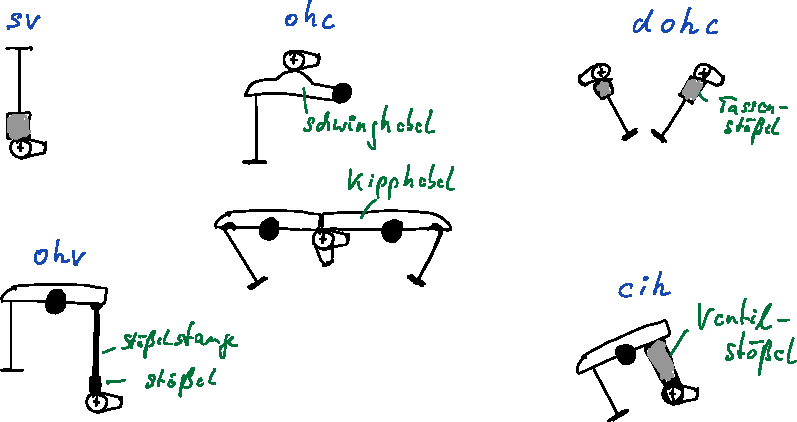
\includegraphics[width=0.6\textwidth]{images/Skizze/01_Anordnung-der-Nockenwelle_Skizze.pdf}
\caption{Anordnung der Nockenwelle}
%\label{fig:}%% anpassen
\end{figure}

\subsection{sv-Motor}\label{sv-motor}

\begin{itemize}
\item
  >>side valves<< seitlich stehende Ventile
\item
  untengesteuerter Motor
\item
  unten liegende Nockenwelle
\end{itemize}

\subsection{ohv-Motor}\label{ohv-motor}

\begin{itemize}
\item
  >>overhead valves<< hängende Ventile
\item
  obengesteuerter Motor
\item
  unten liegende Nockenwelle
\end{itemize}

\subsection{ohc-Motor}\label{ohc-motor}

\begin{itemize}
\item
  >>overhead camshaft<<
\item
  Nockenwelle über Zylinderkopf
\end{itemize}

\subsection{dohc-Motor}\label{dohc-motor}

\begin{itemize}
\item
  >>double overhead camshaft<<
\item
  zwei Nockenwellen über Zylinderkopf
\end{itemize}

\subsection{cih-Motor}\label{cih-motor}

\begin{itemize}
\item
  >>camshaft in head<<
\item
  Nockenwelle im Zylinderkopf
\end{itemize}

\section{Arten von
Nockenwellenantriebe}\label{arten-von-nockenwellenantriebe}

Fachbuch (\textcite{brand:2020:fachkundeKfz} S. 247)

\begin{enumerate}
\item
  Steuerkette
\item
  Zahnriemen
\item
  Königswelle
\item
  Stirnräder
\item
  Schubstangenmotoren
\end{enumerate}

\section{Nenne Zahnriemen Merkmale (trocken
laufend)}\label{nenne-zahnriemen-merkmale-trocken-laufend}

Fachbuch (\textcite{brand:2020:fachkundeKfz} S. 247)

\begin{itemize}
\item
  geringe Masse
\item
  geräuscharmer Lauf
\item
  begrenzte Standzeit, begrenzte Belastbarkeit
\item
  Unterliegen einem Wartungsintervall
\item
  braucht keine Schmierung
\item
  kostengünstig in der Produktion
\item
  Chemisch sensibel
\end{itemize}

\section{Ölbadzahnriemen Eigenschaften (nass
laufend)}\label{oelbadzahnriemen-eigenschaften-nass-laufend}

\begin{itemize}
\item
  mit Öl geschmierter Lauf
\item
  geringere Geräuschentwicklung
\item
  geringere Reibung ($20~\%$ weniger als Steuerkette)
\end{itemize}

\textbf{Ziel:}

\begin{itemize}
\item
  Kontaktflächen der beweglichen Teile reduzieren $\to$ Emissionen
\item
  Thermomanagement: Betriebstemperatur lange halten (BMW)
\end{itemize}

\section{Steuerkette Merkmale}\label{steuerkette-merkmale}

\begin{enumerate}
\item
  Große Kräfte übertragen
\item
  eigentlich wartungsarm, aus praktischer Sicht leider problembehaftet
\item
  teuer in Konstruktion
\item
  Steuerkette gilt als lauter
\item
  größere Masse als ein Riemen
\end{enumerate}

\section{Stirnradantrieb}\label{stirnradantrieb}

\begin{itemize}
\item
  Große Kräfte übertragen
\item
  wartungsfrei
\item
  schmale Bauform
\item
  teuer in Konstruktion
\item
  Dauerläufer (nicht problembehaftet)
\end{itemize}

\section{Königswelle}\label{koenigswelle}

\begin{itemize}
\item
  wartungsfrei
\item
  leicht, weil hohl gebohrt, Hohlröhre
\item
  kleine Kräfte übertragen
\item
  teuer in Konstruktion und Herstellung
\end{itemize}

\section{Unterschied - Steuern und
Regeln}\label{unterschied-steuern-und-regeln}

\subsection{Steuern}\label{steuern}

Soll-Ist-Vergleich

\begin{enumerate}
\def\labelenumi{\alph{enumi}.}
\setcounter{enumi}{25}
\item
  B. \emph{Steuerriemen}: Markierung soll auf OT stehen, alles in
  Ordnung, wenn nicht, dann defekt.
\end{enumerate}

\subsection{Regeln}\label{regeln}

Soll-Ist-Vergleich mit der Option des Eingriffs

\begin{enumerate}
\def\labelenumi{\alph{enumi}.}
\setcounter{enumi}{25}
\item
  B. \emph{ABS Regelkreis}: SG erfasst Drehzahlsignal, Drehen alle Räder
  gleich schnell, alles okay. Dreht ein Rad schneller $\to$ aktiver
  Eingriff ins System.
\end{enumerate}

\section{Nockenwellen -
Herstellungsmöglichkeiten}\label{nockenwellen-herstellungsmoeglichkeiten}

\subsection{Gegossene Nockenwelle}\label{gegossene-nockenwelle}

\begin{itemize}
\item
  muss nachgearbeitet werden, Lagerstellen, partiell gehärtet
\item
  biegsam, flexibles Bauteil (Gusseisen mit Lamellen- o. Kugelgrafit)
\item
  \emph{Vorteil} kostengünstig in der Herstellung, weniger
  problembehaftet
\end{itemize}

(\emph{Kaltverformen} je härter ein Material, um zu spröder.)

\subsection{Gebaute Nockenwelle}\label{gebaute-nockenwelle}

\begin{itemize}
\item
  zwei unterschiedliche Materialien,
\item
  Nocken (aus Einsatz-, Vergütungs- o. Nitrierstahl) auf ein Stahlrohr
  geschrumpft
\item
  \emph{Problem} Nocken können sich verdrehen
\item
  \emph{Vorteil} Gewichtsreduzierung, Nocken ist belastbarer
\item
  \emph{Nachteil} Aufwand
\item
  Material V4A (hohl gebohrt)
\end{itemize}

\section{Nockenformen}\label{nockenformen}

Fachbuch (\textcite{brand:2020:fachkundeKfz} S. 246)

\begin{figure}[!ht]% hier: !ht
\centering
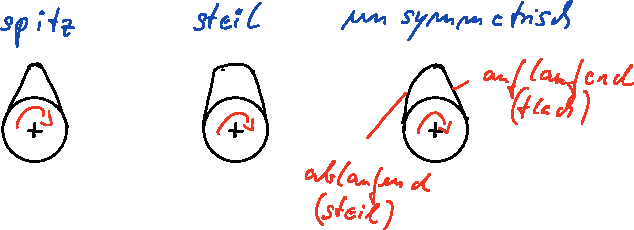
\includegraphics[width=0.6\textwidth]{images/Skizze/02_Nockenformen_Skizze.pdf}
\caption{Nockenformen}
%\label{fig:}%% anpassen
\end{figure}

\subsection{spitzer Nocken (tagenden
Nocken)}\label{spitzer-nocken-tagenden-nocken}

\begin{itemize}
\item
  langsames Öffnen / Schließen der Ventile
\item
  kurze Zeit voll geöffnet\\
\item
  geringe Füllung
\item
  stabiler Leerlauf
\item
  weicher und komfortorientierte Drehzahlbereich
\item
  nicht als hochdrehender, hochbelasteter Motor geeignet
\end{itemize}

\subsection{steiler Nocken (scharfer Nocken, Kreisbogen
Nocken)}\label{steiler-nocken-scharfer-nocken-kreisbogen-nocken}

\begin{itemize}
\item
  schnelles Öffnen / Schließen der Ventile
\item
  bleibt längere Zeit voll geöffnet
\item
  hoher Füllungsgrad, bei hohen Drehzahlen
\item
  im Leerlauf teilweise unrunder Lauf, da >>inneres AGR<< entstehen kann
  (große Ventilüberschneidung $\to$ Abgase in Ansaugtrakt) Abhilfe:
  Leerlaufdrehzahl erhöhen (750 $\to$ 950 U/min.)
\item
  Leistungsmotoren, hohe Drehzahlen
\end{itemize}

\subsection{unsymmetrischer Nocken}\label{unsymmetrischer-nocken}

\begin{itemize}
\item
  \emph{flach} langsameres öffnen der Ventile
\item
  \emph{steil} schnelles schließen der Ventile
\item
  längeres offen halten der Ventile
\item
  vereinigt beide Varianten
\end{itemize}

(\emph{Ziel bei hohen Drehzahlen}: Ventile schnell öffnen (Nocken) /
schließen (Ventilfeder) $\to$ gute Füllung, hohen Wirkungsgrad
erreichen.)

\section{Arten von
Ventilbetätigung}\label{arten-von-ventilbetaetigung}

Fachbuch (\textcite{brand:2020:fachkundeKfz} S. 247, 242)

\begin{figure}[!ht]% hier: !ht
\centering
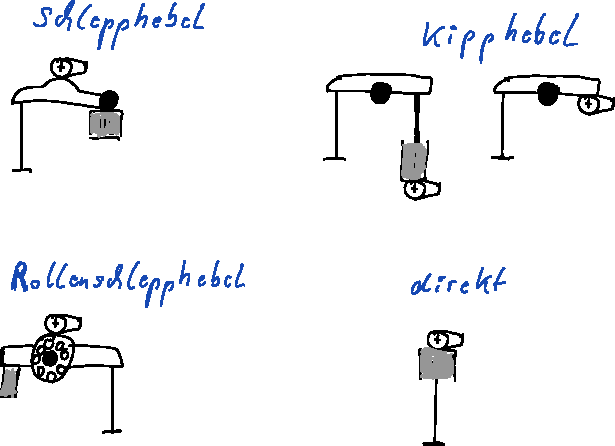
\includegraphics[width=0.6\textwidth]{images/Skizze/03_Arten-von-Ventilbetaetigung_Skizze.pdf}
\caption{Arten von Ventilbetätigung}
%\label{fig:}%% anpassen
\end{figure}

\subsection{Rollenschlepphebel, Schlepphebel,
Schwinghebel}\label{rollenschlepphebel-schlepphebel-schwinghebel}

\begin{itemize}
\item
  einarmige Hebel
\item
  geringe Reibung zwischen Nocken und Schlepphebel durch Nockenrolle
  (nadelgelagert)
\end{itemize}

\subsection{Kipphebel}\label{kipphebel}

zweiarmige Hebel

\subsection{direkt}\label{direkt}

Nockenwelle - Hydrostößel - Ventil

\section{Welche Beanspruchung ist das Ventil
ausgesetzt?}\label{welche-beanspruchung-ist-das-ventil-ausgesetzt}

\subsection{Mechanische Beanspruchung des
Ventils}\label{mechanische-beanspruchung-des-ventils}

\begin{itemize}
\item
  Ziehen (Ventilfeder, schließen, Ventilsitz)
\item
  Druck (Nocken, öffnen)
\item
  Torsion (verdrehen)
\item
  Biegen
\end{itemize}

\subsection{Chemische Beanspruchung}\label{chemische-beanspruchung}

Schwefel im Kraftstoff $\to$ Korrosion

\subsection{Thermische Belastung}\label{thermische-belastung}

Auslassventil bis $900^\circ\text{C}$

\section{Ventilspielausgleich}\label{ventilspielausgleich}

\textbf{Wofür?} Temperaturänderung (Motor Kaltstart, temperaturbedingte
Längenänderung des Ventils ausgleichen)

\textbf{Zu kleines Ventilspiel} (Nachteile)

\begin{itemize}
\item
  Ventil öffnet früher und schließt später
\item
  Ventil ist länger auf
\item
  kann dadurch nicht genügend Wärme abgeben über Ventilsitz
\item
  Ventilteller wird immer weiter einer höheren thermischen Belastung
  unterzogen und dadurch erhöhter Verschleiß
\item
  Am Ende ist das Ventil einer Hochtemperaturkorrosion unterworfen
  (Verbranntes Ventil)
\end{itemize}

\textbf{zu großes Ventilspiel} (Nachteile)

\begin{itemize}
\item
  Ventil öffnet zu spät, geht nicht ganz auf und schließt zu früh
\item
  Ventil ist kürzer auf
\item
  Klappergeräusche und erhöhter Verschleiß, \emph{Warum?} durch großes
  Ventilspiel, liegt nicht am Nockengrundkreis auf (Nocken schlägt auf
  Ventil)
\item
  Hieraus können folgen: schlechte Zylinderfüllung und die maximale
  erreichbare Leistung sinkt
\end{itemize}

\subsection{definiertes Ventilspiel}\label{definiertes-ventilspiel}

Wartung notwendig

\subsection{Hydraulischer
Ventilspielausgleich}\label{hydraulischer-ventilspielausgleich}

\textbf{ablaufender Nocken} (ohne Belastung)

\begin{itemize}
\item
  Entspannung des Systems
\item
  Spielausgleichsfeder drückt Druckbolzen nach oben bis Stößel am Nocken
  anliegt
\item
  Kugelventil öffnet sich, Raumvergrößerung im Arbeitsraum (Unterdruck)
\item
  Durch den Systemdruck strömt frisches Öl von außen ein und der
  Arbeitsraum wird befüllt
\end{itemize}

\textbf{auflaufender Nocken} (mit Belastung)

\begin{itemize}
\item
  Kugelventil schließt sich, es baut sich Druck im System auf
\item
  durch die Inkompressibilität von Flüssigkeiten $\to$ starre
  Verbindung
\item
  Nocken wird auf den Stößel auflaufen können, ohne Spiel zu haben und
  das Ventil betätigen
\item
  \emph{Warum Ringspalt?} (Wärmeausdehnung des Öls ausgleichen)
\item
  Wärmeeintrag: je wärmer das Öl, umso dünnflüssiger
\item
  dadurch wird >>Öl<< durch den kleinen Ringspalt gepresst (definierte
  Menge an Öl)
\item
  erfordert die richtige Öl-Viskosität (Zähflüssigkeit,
  Temperaturabhängig, Fließverhalten), sind an diese Ringspalte
  angepasst
\end{itemize}

Fachbuch (\textcite{brand:2020:fachkundeKfz} S. 245)

\begin{figure}[!ht]% hier: !ht
\centering
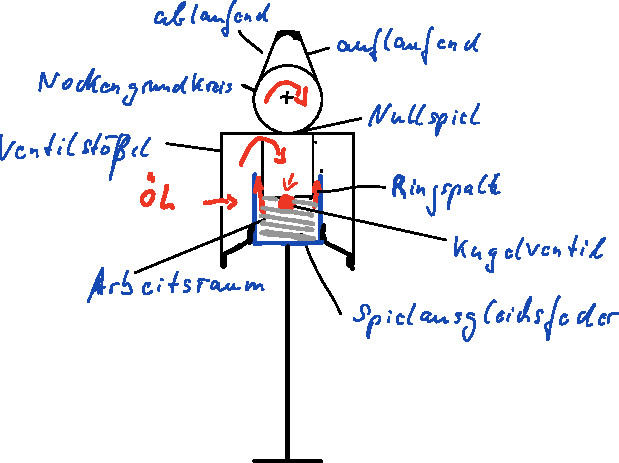
\includegraphics[width=0.6\textwidth]{images/Skizze/04_Ventilspielausgleich_Skizze.pdf}
\caption{Ventilspielausgleich}
%\label{fig:}%% anpassen
\end{figure}

\section{Drehzahlverhältnis zwischen Kurbelwelle zu
Nockenwelle?}\label{drehzahlverhaeltnis-zwischen-kurbelwelle-zu-nockenwelle}

2:1

\section{Was steuert die
Motorsteuerung?}\label{was-steuert-die-motorsteuerung}

Den Zeitpunkt und die Dauer des Ansaugens der Frischgase und den
Zeitpunkt und die Dauer des Ausstoßes der Abgase.

Öffnen und Schließen der Ventile.

\textbf{Voraussetzung}

\begin{enumerate}
\item
  Einspritzung des Kraftstoffs (Energieträger)
\item
  Eine Zündung, die diese Energie, gebunden im Kraftstoff, in chemische
  Energie, in Wärmeenergie umwandelt (Wärmekraftmaschine)
\end{enumerate}

Druck wird über eine Fläche in Kraft und Drehmoment übertragen, an die
Kurbelwelle übergeben, läuft durch das Getriebe - Achswellen - Reifen
auf die Straße und wir haben Vortrieb.

\section{Dreiventiltechnik mit zwei
Zündkerzen}\label{dreiventiltechnik-mit-zwei-zuendkerzen}

Fachbuch (\textcite{brand:2020:fachkundeKfz} S. 243)

Fachbuch (\textcite{respondeck:2019:servicetechniker} S. 142)

\subsection{Zusammenfassung}\label{zusammenfassung}

\begin{figure}[!ht]% hier: !ht
\centering
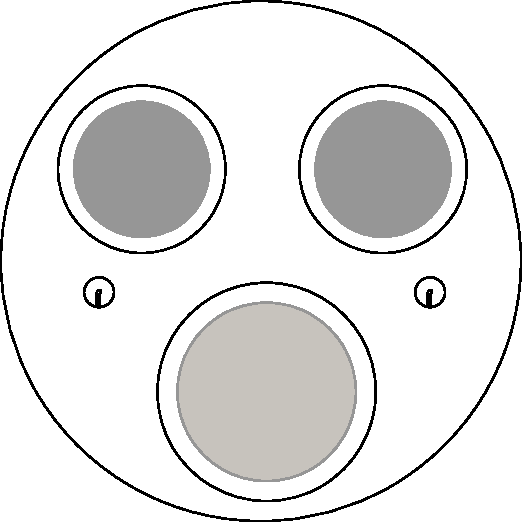
\includegraphics[width=0.2\textwidth]{images/Skizze/05_Dreiventiltechnik_Skizze.pdf}
\caption{Dreiventiltechnik}
%\label{fig:}%% anpassen
\end{figure}

Wir haben bei \textbf{drei Ventilen} einen großen Ein- und
Auslassquerschnitt.

Durch die Anordnung ist eine Unterbringung von \textbf{zwei Zündkerzen}
möglich, sodass zwei Zündkerzen in der Nähe der Zylinderwand entstehen
in deren Umgebung zwei Flammfronten. Somit kann bereits
niedergeschlagener Kraftstoff noch verdampfen und verbrannt werden.

Durch zwei Zündkerzen findet die Verbrennung schneller statt. Dadurch
wird der maximale Kolbendruck früher erreicht und ein hohes Drehmoment
erreicht. Wir nähern uns einer Gleichdruckverbrennung (Isobar).

\textbf{Klopfneigung} wird durch zwei Zündkerzen verringert. Da
geringere Wärmeeintrag in die noch nicht verbrannten Gase stattfindet.

\textbf{Abgastemperatur} ist niedriger, dadurch geringerer NOx-Ausstoß
trotz geringer HC und CO-Werte.

Dank nur \textbf{einem Abgasrohr} geringere Wärmeverluste. >>light off
point<< des Katalysators wird schneller erreicht.

\subsection{Warum sind das zwei Einlassventile und ein
Auslassventil?}\label{warum-sind-das-zwei-einlassventile-und-ein-auslassventil}

\textbf{Vorteil}

\begin{itemize}
\item
  kleine Massen
\item
  zwei kleine Ventile $\to$ große Einlassquerschnitte
\item
  höhere Drehzahlen
\item
  gute Füllung und Zylinderspülung
\end{itemize}

\textbf{Nachteil}

\begin{itemize}
\item
  mehr Teile $\to$ größere Reibungsverluste
\item
  Verschleiß und Ausfallwahrscheinlichkeiten
\end{itemize}

\textbf{Ein großes Ventil} hat eine Massenträgheit.

\begin{itemize}
\item
  Masse in Ruhelage (Ventil offen), Losbrechmoment~ $\to$ höchste
  Kraft, Masse in Bewegung (Federkraft: Ventil schließen)
\item
  Ansaugventil möglichst lange offen lassen (Kolben und Ventil kommen
  sich sehr nahe)
\item
  \emph{Ziel:} bestimmte Drehzahl erreichen (Wie schnell kann dieser
  Wechsel vollzogen werden?)
\end{itemize}

\subsection{Zylinderspülung bei
Ventilüberschneidung}\label{zylinderspuelung-bei-ventilueberschneidung}

Mit dem Ausstoß der Abgase ziehen wir einen kleinen definierten
Frischgasanteil mit, um den Zylinder zu spülen und möglichst wenig
inertes Gas (AGR) zu gewährleisten.

\subsection{Nachladeeffekt beim
Ansaugen}\label{nachladeeffekt-beim-ansaugen}

Einlassventile werden erst nach Durchschreiten des unteren Totpunktes
geschlossen. Frischgase strömen trotz aufwärtsgehendem Kolben in den
Zylinder nach. Die Kinetische Energie der einströmenden Frischgase ist
größer, als die Druckzunahme durch aufwärts gehenden Kolben.

\subsection{Warum zwei Zündkerzen?}\label{warum-zwei-zuendkerzen}

Zündkerze ist in der Nähe der Zylinderwand, zwei Flammenfronten
entstehen.

\begin{enumerate}
\item
  \textbf{Vollständige Verbrennung}

  \begin{itemize}
  \item
    niedergeschlagener Kraftstoff verdampft (an Zylinderwandung und
    Feuersteg) und der Verbrennung zugeführt
  \end{itemize}
\item
  \textbf{schnellerer Verbrennungsablauf}

  \begin{itemize}
  \item
    Schnelleres erreichen des maximalen Verbrennungsdruckes. Die
    Temperatur kann schneller konstant gehalten bzw. in Druck
    umgewandelt und über die Fläche des Kolbens in Kraft und Drehmoment
    auf die Kurbelwelle übertragen werden.
  \item
    Drehmoment = Kraft (max. Kolbendruck) x Hebelarm (90° stehende
    Kurbelwellenzapfen = Hebelarm am größten)
  \end{itemize}
\end{enumerate}

\subsection{Innermotorisch entstehen geringere
Schadstoffe}\label{innermotorisch-entstehen-geringere-schadstoffe}

\begin{enumerate}
\item
  \textbf{HC} geringer Ausstoß unverbrannter Kohlenwasserstoffe, durch
  weniger niedergeschlagener Kraftstoff
\item
  \textbf{CO} geringer, durch vollständige Verbrennung
\item
  \textbf{NOx} ist reduziert, durch schnelleren Verbrennungsablauf
  $\to$ zwei Zündkerzen, Abgastemperatur ist niedriger
\end{enumerate}

\subsection{Wann entsteht NOx?}\label{wann-entsteht-nox}

Durch hoher Druck und hohe Temperatur.

\subsection{Zusammenhang zwischen HC und CO
vs.~NOx}\label{zusammenhang-zwischen-hc-und-co-vs.-nox}

Es gibt zwei Zündgrenzen >>fett<< und >>mager<<.

\begin{enumerate}
\item
  \textbf{HC und CO} entsteht durch unvollständige fette Verbrennung

  \begin{itemize}
  \item
    Senken: durch Abmagern
  \item
    Verbrennungsspitzentemperatur: geringer
  \end{itemize}
\item
  \textbf{NOx} entsteht durch magere Verbrennung

  \begin{itemize}
  \item
    Senken: durch anfetten
  \item
    Verbrennungsspitzentemperatur: ansteigen
  \end{itemize}
\end{enumerate}

\subsection{Schadstoffe}\label{schadstoffe}

\begin{enumerate}
\item
  \textbf{HC} unverbrannte Kohlenwasserstoffe

  \begin{itemize}
  \item
    Verdampft am Ende der Verbrennung und wird dem Abgas zugeführt
  \end{itemize}
\item
  \textbf{CO} Kohlenmonoxid

  \begin{itemize}
  \item
    schwerer als Luft (Grube), bindet Hämoglobin im Blut
  \item
    keine vollständige Verbrennung
  \end{itemize}
\item
  \textbf{NOx} Stickoxide
\end{enumerate}

\subsection{Was ist AGR?}\label{was-ist-agr}

Platzhalter Gas (inertes Gas) nimmt nicht an der Verbrennung teil, soll
den Umgebungssauerstoff fernhalten

AGR-Rate ist am größten in Teillast (80 Km/h auf der Landstraße)

Ziel: Aus großen Motor $\to$ kleinen Motor machen, viel Abgas und
geringe Menge Kraftstoff einspritzen

\emph{Problem} >>Luftmenge ist da und kein Kraftstoff Einspritzen<<
$\to$ magere Verbrennung $\to$ thermische Belastung und Anstieg NOx

\emph{Luftmassenmesser} misst angesaugte Luftmasse und Sauerstoffgehalt
$\to$ AGR-Rate $\to$ Kraftstoffmenge berechnen

Ziel: homogen - Magerbetrieb (über den kompletten Zylinder)

\subsection{Wie entsteht Ruß?}\label{wie-entsteht-russ}

Kraftstoff wird an heißen Luft eingespritzt, zündfähiges
Kraftstoff-Luft-Gemisch bildet sich

\emph{einzelne Kraftstofftröpfchen}

\begin{itemize}
\item
  fangen von außen an zu verdunsten, entzünden, Verbrennung ist zu kurz
  (nicht vollständig)
\item
  innen: Verbrennung von Kohlenwasserstoff ohne Sauerstoff
\end{itemize}

\subsection{Was fördert die
Klopfneigung?}\label{was-foerdert-die-klopfneigung}

Unkontrollierte, unerwünschte Verbrennung (Glühzündung, klingende,
klopfende Verbrennung)

entzündet sich selbst an etwas glühenden, z. B. Ölkohle, Masseelektrode
(Zündkerze)

Wärme braucht Zeit zum Wirken.

\begin{enumerate}
\item
  \textbf{Wärmeeintrag gering:} geringe Klopfneigung, geringe thermische
  Belastung, schneller Verbrennungsablauf
\item
  \textbf{Wärmeeintrag hoch:} klopfende Verbrennung
\end{enumerate}

\subsection{Ein Auslassventil - ein
Abgasrohr}\label{ein-auslassventil-ein-abgasrohr}

Abgas verliert weniger Wärmeenergie.

\begin{enumerate}
\item
  ab ca. 450~°C >>light off point<< des Katalysators: min. $50~\%$ der
  Abgase konvertiert in nicht Schadstoffen
\item
  ab ca. 650 °C altert der Katalysator exponentiell und thermische
  Belastung
\end{enumerate}

\textbf{Thermodynamik - warme Luft strömt} schneller, weniger Rückstau.

Das unter Druck stehende Abgas verlässt den Zylinder mit Überschall
(Auspuffgeräusch). \textbf{Schallgeschwindigkeit} ca. 343 m/s (z. B.
Blitz $\to$ Donner, drei Sekunden zählen $\to$ ca. 1 km Entfernung)


	%%%%%%%%%%%%%%%%%%%%%%%%%%%%%%%%%%%%%%%%%%%%%%%%%%%%%%%%%%%%%%%%%%
    % Bibliographie
    \printbibliography[category=cited]
\end{document}
